\section{Method}

\todo{%
\begin{itemize}
    \item intuition behind distances -> positions?
    \item explain the maps (Euler/quaternion -> SO(3)) more, give intuition why quaternions are better
    \item sampled sum
\end{itemize}
}

% \lau{Lau: As far as I'm concerned, everything below before subsection 2.1 could also go at the end of the Introduction. Beyond the fact that it contains literature review and conceptual information that would go well in the intro, I find the current architecture of Section 2 a bit puzzling. First there is text to explain the methods and detail their intuition/key components, then there are three consecutive subsections that kind of do the same, but from a maths points of view. The aforementioned suggestion of putting the first text in the intro could solve this. Another possibility: put the descriptive texts in their corresponding sub-sections, so that those contain both the motivation and the maths. I'm open to further suggestions and suggestions ;-) }
% \mdeff{Indeed. The "Distance Learning" and "Orientation Recovery" paragraphs might go in their respective sub-sections. But I'd like to keep a high-level motivation of the whole method (the text linked to the second figure to appear alongside \figref{imaging-geometry}.}
% \lau{Fine for me.}
% \banjac{I moved the DE and OR to corresponding subsections. The short intro to methods I left here at the beginning of the section 2 (I didn't move it to intro). Let me know if you meant something different}

\begin{figure}
    \centering
    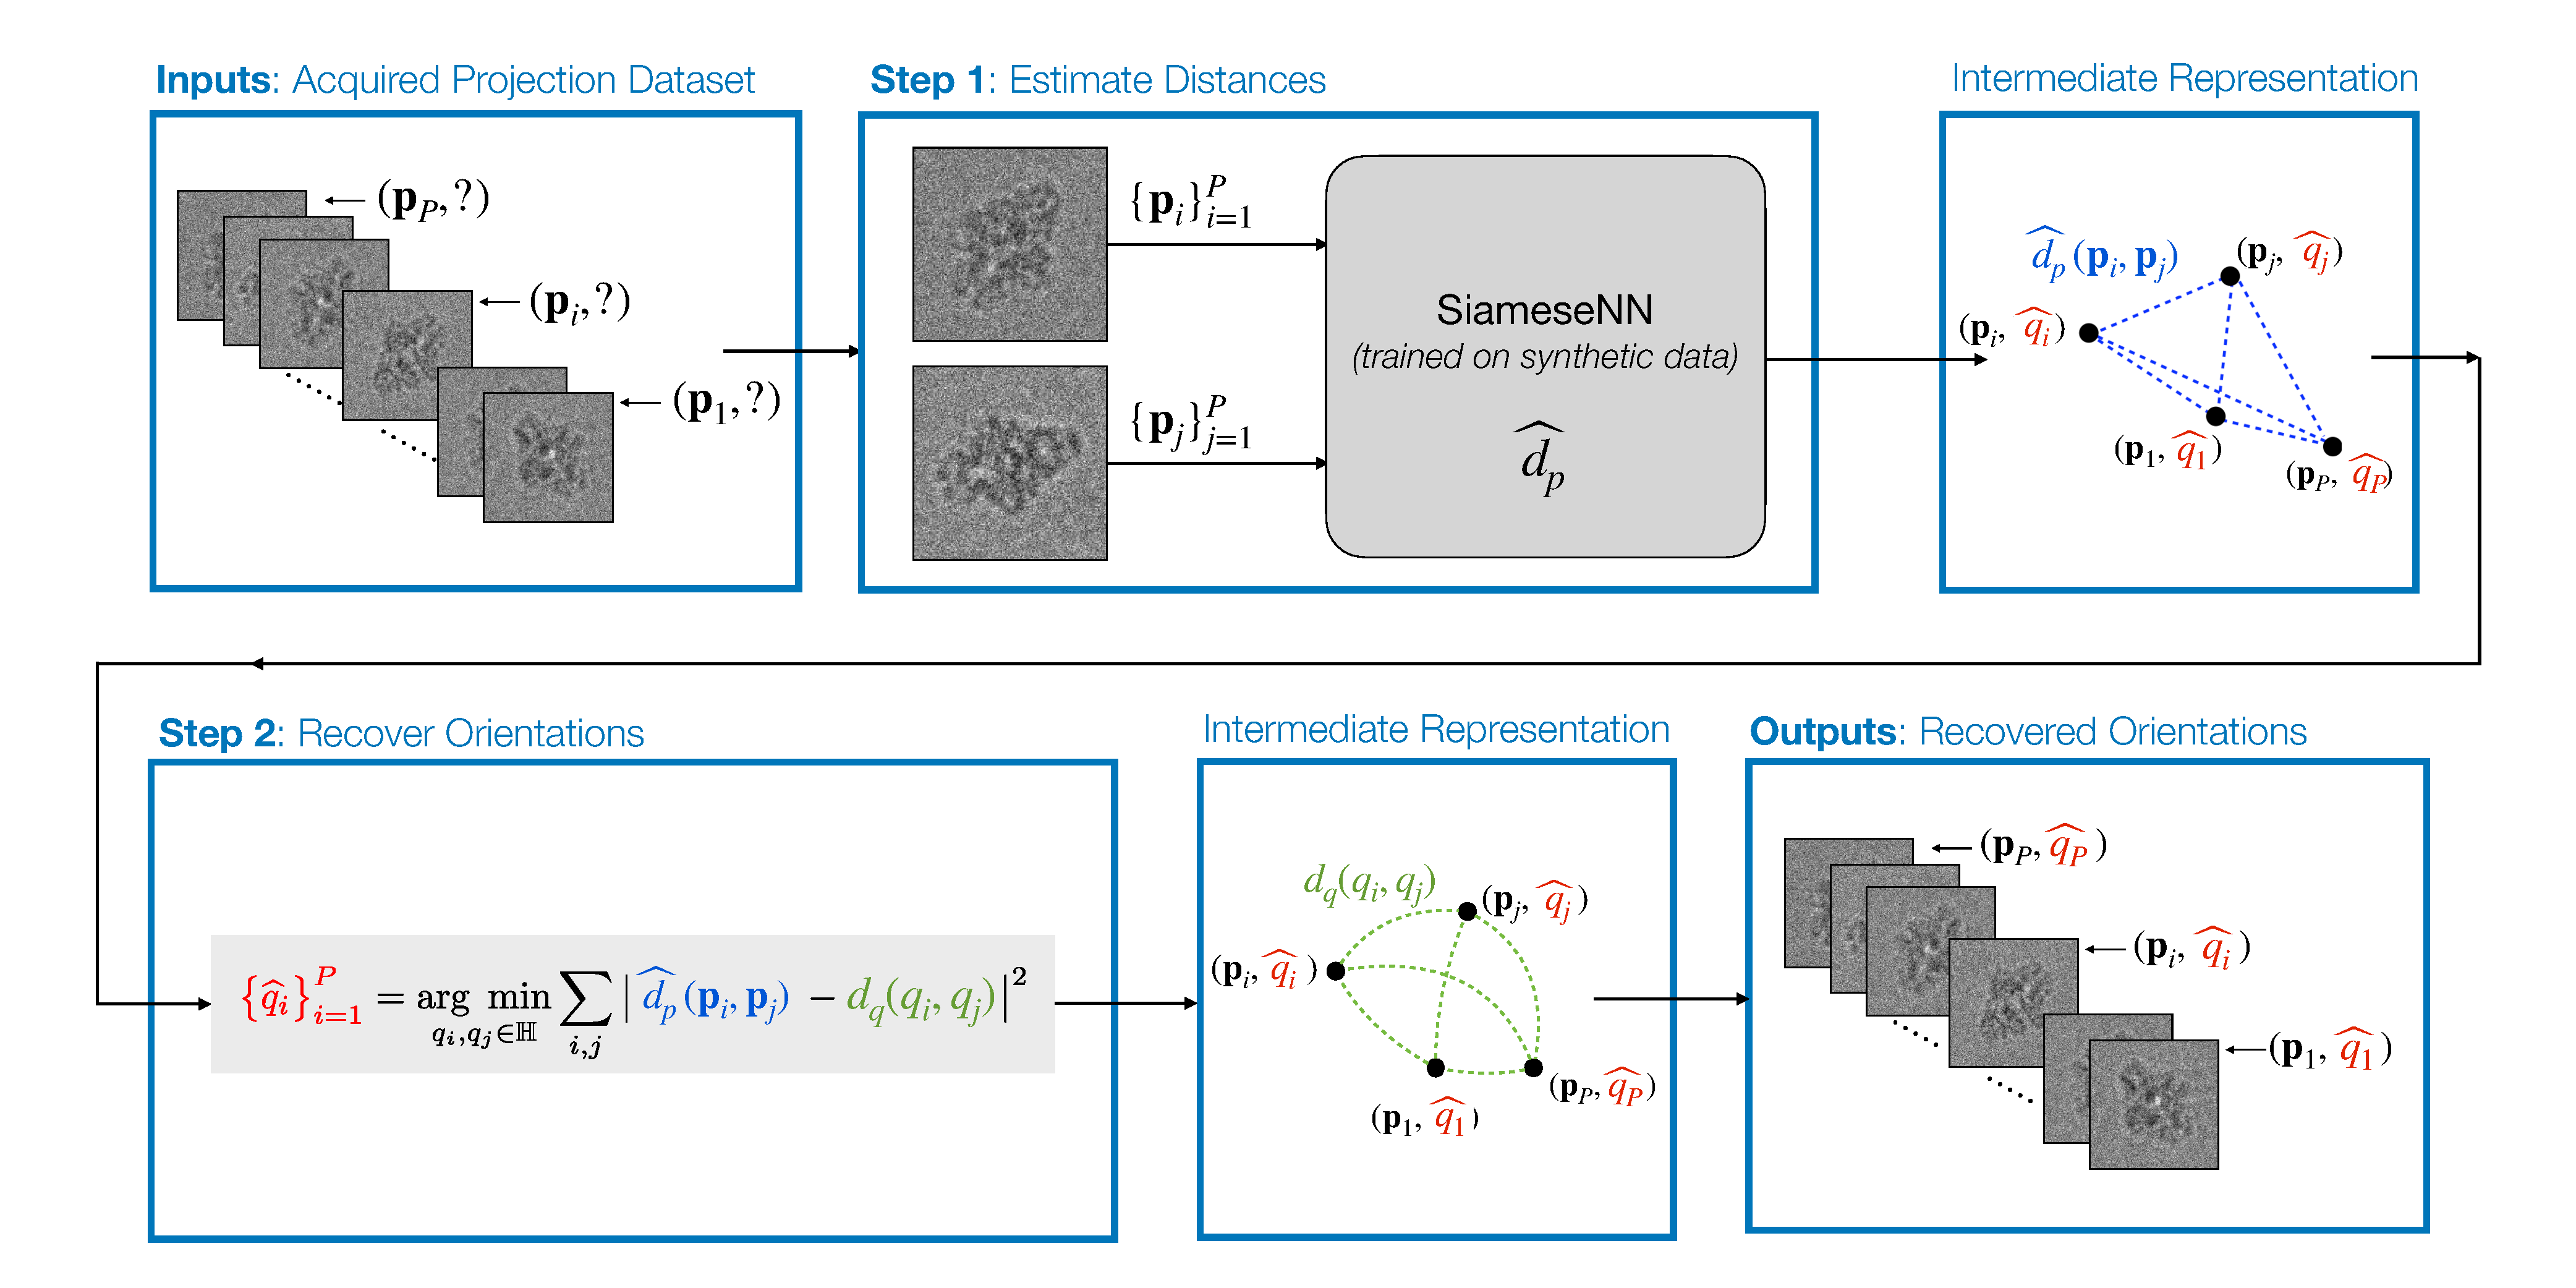
\includegraphics[width=\linewidth]{schematic_method_overview}
    \caption{%
        %\textbf{Method:}
        Our method consists of two steps.
        First, we estimate distances between pairs of projections.
        Second, we recover the orientation of each projection from these distances.
    }\label{fig:schematic:method-overview}
\end{figure}

Our approach relies on two observations (\figref{intuition-method}), yielding two steps (\figref{schematic:method-overview}).
First, the greater the similarity between two 2D projections $(\p_i, \p_j)$, the more likely they originated from two 3D particles that adopted close orientations $(q_i, q_j)$ in the ice layer prior to imaging;\footnote{Up to protein symmetries, which we discuss later.} this observation guides a number of applications in the field~\cite{frank2006three}.
% TODO: differences in orientation / distances
Hence, we aim to estimate differences in orientation $d_q(q_i, q_j)$ from the projections themselves as $\widehat{d_p}(\p_i, \p_j)$ (\secref{method:distance-learning}).
% where $\widehat{d_p}$ is learned from training data
\todo{Second, orientations are constrained by their relative differences.}
Second, we can learn the projection manifold by finding the distances that preserves the geometry of local neighborhoods in the space of orientations.
Hence, from a set of projections $\{\p_k\}_{k=1}^P$, we aim to recover their orientations $\{\widehat{q_k}\}_{k=1}^P$ such that the induced distances $d_q(\widehat{q_i}, \widehat{q_j})$ are close to the estimated distances $\widehat{d_p}(\p_i, \p_j)$ (\secref{method:orientation-recovery}).
All in all, $d_q(q_i, q_j) \approx \widehat{d_p}(\p_i, \p_j) \approx d_q(\widehat{q_i}, \widehat{q_j})$, with equality if $\widehat{d_p}$ and $\{\widehat{q_k}\}_{k=1}^P$ are perfectly estimated.

\lau{Moved from Appendix}. \lau{Jelena: What you observed when trying that.}
% it could be tempting to
Note that an alternative could have been to train $\mathcal{G}_w$ to directly map projections to orientations, i.e., $\widehat{q_i} = \mathbf{f}_i = \mathcal{G}_w(\p_i)$, hence avoiding the orientation recovery step.
While that solution is simpler, learning an embedding in a space of $n_f \gg 4$ dimensions gives enough room for $\mathcal{G}_w$ to represent different proteins, noise levels, PSFs, etc., which are then abstracted by taking distances.
% $n_f=4$ dimensional space is too constrained
\mdeff{Did we try that? Would be nice to have the results if we did.}

%We propose to learn a function---parametrized as a neural network---to predict the relative orientation between two projections based on their similarity.
%This distance function then allows us to estimate, for any new projection dataset, the relative orientations between pairs of projections.

% Our method effectively (i) estimates a metric space, then (ii) embed/realize it in the space of 3D orientations, $\SO(3)$.

%Given sufficiently many and accurate estimations
%If the distances are exact geodesic distances between orientations, then orientation recovery will find a perfect realization of the metric space, with zero error.
%In practice, distances estimated from projections will only be a proxy of true distances.
%Experiment \secref{results:orientation-recovery:sensitivity} shows that a lower distance estimation error translates to a lower orientation recovery error.

%\subsection{Unit Quaternions and the Geodesic Distance}
%\subsection{Parameterization of orientations}
\subsection{Representation of orientations with quaternions}\label{sec:method:orientation-representation}
%\subsection{Orientations and distances}\label{sec:method:orientation-representation}
%\subsection{Distance between orientations}
%\mdeff{Laurène: Which word is better: Representation or parameterization? Or something else, but we need consistency.}
%\lau{Both are fine. Personally, I use parametrization in my thesis, but we can settle on the other one.}
% representation of orientations, parameterization of rotation matrices

%The projection $\mathbf{P}_{\bth}$ in \eqnref{imaging-model} represents an integration through the 3D particle made by the beam of electrons.
The orientation of a 3D particle with respect to the microscope's detector plane is a rotation relative to a reference orientation (\figref{imaging-geometry}).
The group of all 3D rotations under composition is identified with $\SO(3)$, the group of $3 \times 3$ orthogonal matrices with determinant~1 under matrix multiplication.
% non-commutative/non-Abelian\footnote{order of rotations matter}
A rotation matrix $\mathbf{R}_{\bth} \in \SO(3)$ can be decomposed as a product of $\binom{3}{2}=3$ independent rotations, for example as $\mathbf{R}_{\bth} = \mathbf{R}_{\theta_3} \mathbf{R}_{\theta_2} \mathbf{R}_{\theta_1}$, where $\bth = (\theta_3,\theta_2,\theta_1) \in [0,2\pi[ \, \times \, [0,\pi] \times [0,2\pi[$ are the (extrinsic and proper) Euler angles in the $ZYZ$ convention (a commonly-used parameterization in cryo-EM)~\cite{sorzano2014interchanging}.
%As illustrated in \figref{imaging-geometry}, $\mathbf{R}_{\theta_1}$ is a rotation about the $Z$-axis by the angle $\theta_1$, $\mathbf{R}_{\theta_2}$ is a rotation about the $Y$-axis by the azimuthal (or tilt) angle $\theta_2$, and $\mathbf{R}_{\theta_3}$ is a second rotation about the $Z$-axis by the in-plane angle $\theta_3$.
%The Euler angles $\bth$ and the rotation matrix $\mathbf{R}_\bth$ are equivalent representations of the orientation of a projection.

While Euler angles are a concise representation of orientation ($3$ numbers for $3$ degrees of freedom), they suffer from a topological constraint (there is no covering map from the $3$-torus to $\SO(3)$) which manifests itself in the \textit{gimbal lock}, the loss of one degree of freedom when $\theta_2=0$. %~\cite{koks2006explorations}
This makes their optimization by gradient descent (\secref{method:orientation-recovery}) problematic.
On the other hand, the optimization of rotation matrices---made of $9$ numbers---would require computationally costly constraints (orthogonality and determinant~1) to reduce the number of degrees of freedom to $3$.
Moreover, the distance between orientations cannot be directly computed from Euler angles and is costly (30 multiplications) to compute from rotation matrices~\cite{huynh2009metrics}.
We solve both problems by representing orientations with unit quaternions.

%\paragraph{Quaternions.}
Quaternions $q \in \mathbb{H}$ are an extension of complex numbers\footnote{The algebra $\mathbb{H}$ is similar to the algebra of complex numbers $\mathbb{C}$, with the exception of multiplication being non-commutative.} of the form $q = a + b\boldsymbol{i} + c\boldsymbol{j} + d\boldsymbol{k}$ where $a,b,c,d \in \R$.
Unit quaternions $q \in \mathbb{S}^3$, where $\mathbb{S}^3 = \big\{ q \in \mathbb{H}: \lvert q \rvert = 1 \big\}$ is the 3-sphere (with the additional group structure inherited from quaternion multiplication), concisely and elegantly represent a rotation of angle $\theta$ about axis $(x_1, x_2, x_3)$ as $q = \cos(\theta/2) + x_1 \sin(\theta/2) \boldsymbol{i} + x_2 \sin(\theta/2) \boldsymbol{j} + x_3 \sin(\theta/2) \boldsymbol{k}$.
They parameterize rotation matrices as
\begin{equation*}
    \mathbf{R}_q =
    \begin{pmatrix}
        a^2+b^2-c^2-d^2 & 2bc-2ad & 2bd+2ac \\
        2bc+2ad & a^2-b^2+c^2-d^2 & 2cd-2ab \\
        2bd-2ac & 2cd+2ab & a^2-b^2-c^2+d^2
    \end{pmatrix}.
\end{equation*}
%Composition of rotations is given by multiplications of quaternions.
Note that $\mathbb{S}^3 \rightarrow \SO(3)$ is a two-to-one mapping (a double cover) as $q$ and $-q$ represent the same orientation, i.e., antipodal points of $\mathbb{S}^3$ are equivalent.
%\paragraph{Distances.}
Unlike Euler angles, $\mathbb{S}^3$ is isomorphic to the universal cover of $\SO(3)$.
Hence, the distance between two orientations, i.e., the length of the geodesic between them on $\SO(3)$, is given by
\begin{equation}
    \begin{aligned}
        d_q &: \mathbb{S}^3 \times \mathbb{S}^3 \rightarrow [0,\pi], \\
        d_q(q_i, q_j) &= 2 \arccos \left( \left| \langle q_i, q_j \rangle \right| \right),
    \label{eqn:distance:orientations}
    \end{aligned}
\end{equation}
where $\langle \cdot, \cdot \rangle$ is the inner product and the absolute value $\left| \cdot \right|$ ensures that $d_q(q_i, q_j) = d_q(q_i, -q_j)$.
The distance $d_q(q_i, q_j)$ corresponds to the magnitude (angle) of the rotation $\mathbf{R}_*$ such that $\mathbf{R}_{q_i} = \mathbf{R}_* \mathbf{R}_{q_j}$~\cite{huynh2009metrics}.

%For the sake of conciseness, we shall use the term ``with orientation~$q$'' to refer to 2D/3D objects considered in an imaging geometry parametrized by $q$.

% Euler angles:
% - Euler angles are not unique
% - gimbal lock problem
% - intuition behind changing the basis between two coordinate systems is not so clear
% - to compare if 2 different projs are close to each other in their projection directions, it does not suffice comparing their 2 sets of Euler angle sets
% - 3 unknown parameters
% - just used for representation of input and output format of rotation

% Affine transformations / rotation matrices:
% - intuitive
% - unique
% - 3x3 matrix, 9 parameters
% - used for angle alignment due to its transformation versatility (e.g. mirrors)
% simpler to compose
% avoid problem of gimbal lock
%Rotation matrix: Minor disadvantage: Multiplication of matrices is ~2 times slower than quaternions. Minor Advantage: Matrix-vector multiplication is ~2 times faster, and large. Huge disadvantage: Normalization! Ghram-Shmit is asymmetrical, which does not give a higher order accurate answer when doing differential equations. More sophisticated methods are very complex and expensive.

% Quaternions:
% - intuition behind changing the basis between two coordinate systems is not so clear
% - 4D vector, 4 unknown parameters
% - much less known in EM community, but they can be used to describe rotation
% - any time we need to perform rotation on camera position, the quaternion is translated into its corresponding rotation matrix and then it is applied to the coordinates of the central coordinate system
% - mirroring using quaternions - we lose any intuition about how two projection directions (mirrored and non-mirrored) are related
% more compact and numerically stable
%Unfortunately, the intuition behind changing the basis between two coordinate systems is not so clear and performing reflections (also known as mirrors, flips) using quaternions we lose any intuition about how two projection directions (mirrored and non-mirrored) are related.
%However, quaternions are more compact (4D vectors/4 scalars) and numerically stable compared to rotation matrices.
%The quaternions strike a nice balance of both, Euler angles and rotation matrices, being small and free from gimbal lock.

% Axis angles
% - used for visualizations
%Axis (angle = length of axis) Minor advantage: Small. Moderate disadvantage: Multiplication and applying to a vector is slow with trig. Moderate disadvantage: North-pole singularity at length = 2*pi, since all axis directions do nothing. More code (and debugging) to automatically rescale it when it gets near 2pi.

\subsection{Distance learning}\label{sec:method:distance-learning}
%\subsection{Metric learning}%\label{sec:method:distance-learning}
%\subsection{Estimating Relative Orientations from Projections}
%\subsection{Relative orientation estimation}
%\subsection{Relative orientation estimation from projections}

%We aim to learn a function $\widehat{d_p}$---parametrized as a neural network---to predict the relative orientation between two projections based on their similarity.

We aim to estimate a function $\widehat{d_p}$ such that $\widehat{d_p}(\p_i, \p_j) \approx d_q(q_i, q_j)$.
While we could in principle design $\widehat{d_p}$, that would be intricate---if not impossible---partly because the invariants are difficult to specify.
We instead opt to learn $\widehat{d_p}$, capitalizing on (i) the powerful function approximation capabilities of neural networks, and (ii) the possibility to generate realistic cryo-EM projection datasets supported by the availability of numerous 3D atomic models\footnote{\url{https://www.ebi.ac.uk/pdbe/emdb}} and our ability to model the imaging procedure.

\begin{figure}
    \centering
    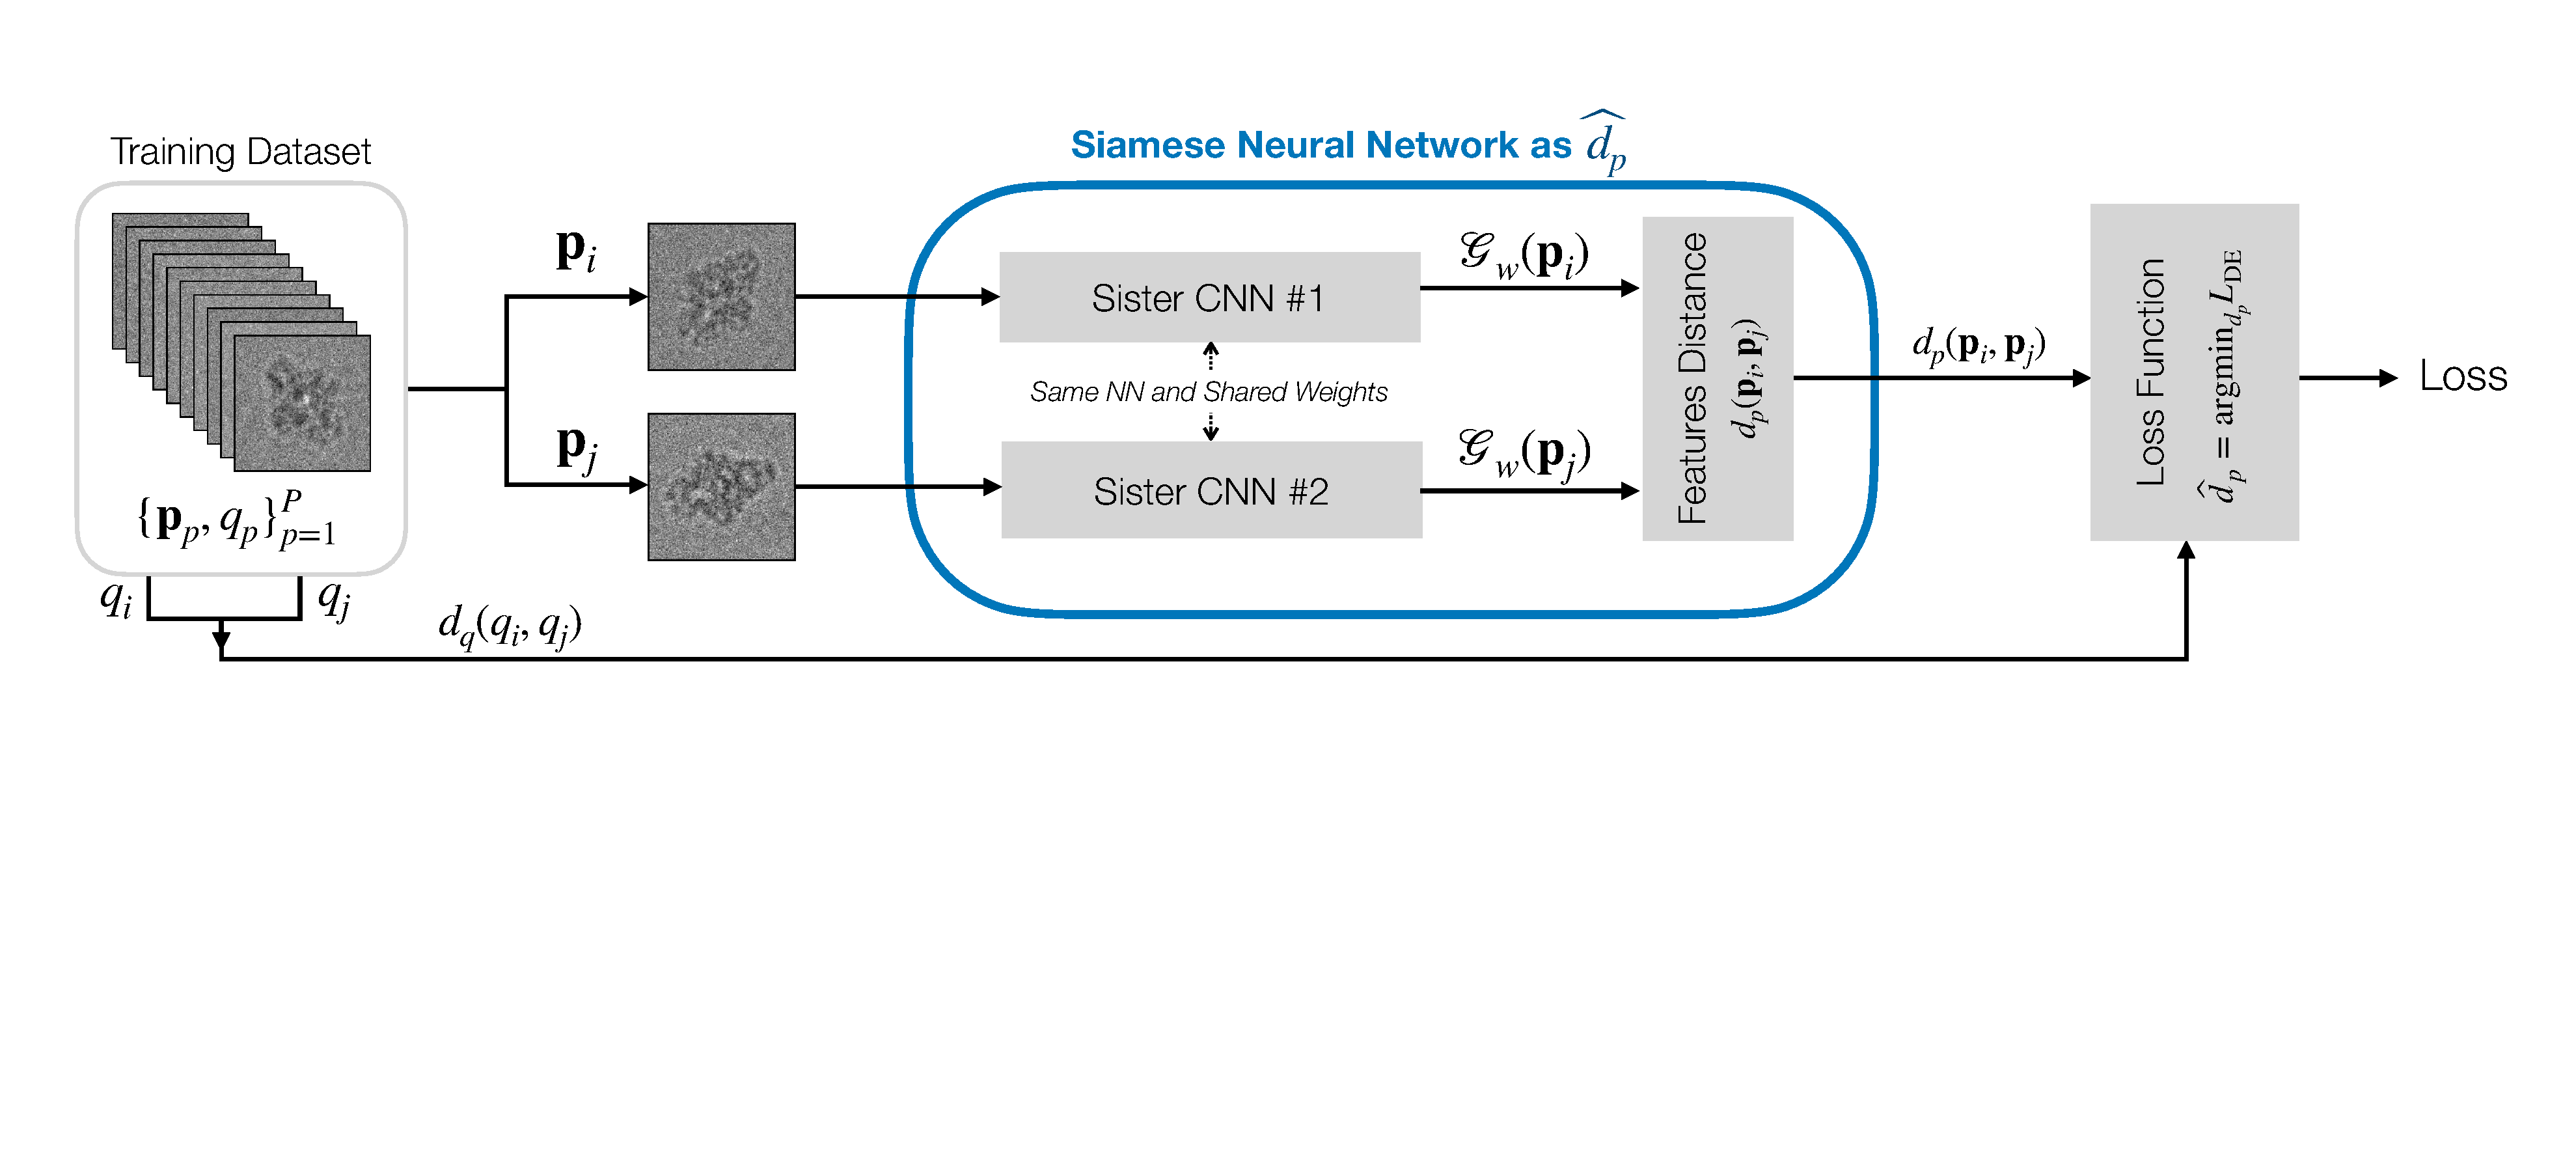
\includegraphics[width=\linewidth]{schematic_distance_learning}
    \caption{%
        \textbf{Distance learning.}
        We are looking for a distance $d_p$ between projections that is an accurate estimator of the distance $d_q$ between their orientations.
        We propose to parameterize $d_p$ as a Siamese neural network (SiameseNN), trained on a synthetic dataset of projections with associated orientation.
        %\mdeff{Why the output "loss" arrow? To me, this system is closed.}
        %\mdeff{"Loss Function" could be called Optimization or Learning or Training.}
}\label{fig:schematic:distance-learning}
\end{figure}

From a training dataset ${\{ \mathbf{p}_{i}, q_i \}}_{i=1}^{P}$, we learn the projection distance
\begin{equation}
    \widehat{d_p} = \argmin_{d_p} L_\text{DE},
    \quad \text{where} \quad
    L_\text{DE} = \sum_{i,j} \left| d_p\big(\mathbf{p}_{i},\mathbf{p}_{j}\big) - d_q\big(q_i,q_j\big) \right|^2
    \label{eqn:distance-learning}
\end{equation}
is the loss and $d_q$ is defined in~\eqnref{distance:orientations}.
The distance $d_p$ is parameterized as the Siamese neural network (SiameseNN)~\cite{chopra2005learning}
\begin{equation*}
    d_p(\p_i, \p_j) = d_f(\G_w(\p_i), \G_w(\p_j)),
    %\label{eqn:distance:projections}
\end{equation*}
where $\G_w$ is a convolutional neural network with weights $w$ that is trained to extract the most relevant features $\f_i \in \R^{n_f}$ from a projection $\p_i$.
\todo{NN architecture constrains (a priori) the function space $\G_w$ is drawn from. Convolution because we want translation invariance (embodiment of prior expert knowledge, generalization guarantee). Ideally we would like noise and PSF invariance too, but those are hard to build in. Hence we resort to data augmentation (i.e., training on perturbed projections).}
\todo{After some experimentation, we ended up with the architecture described in \apxref{siamese-architecture} (for all experiments). While it gave good performance for a reasonable runtime, it can be optimized further. Especially when training on more data (beyond our proof-of-concept).}
% \mdeff{Architecture of $G_w$ doesn't seem to matter much. Surprising, because we don't overfit $\rightarrow$ future research needed.}
%SiameseNNs come with a variety of more or less powerful architectures.
%At the current stage of development, we work with a simple one.
%Our SiameseNN is composed of two convolutional neural networks (CNNs) with shared weights.
%\todo{Jelena: could we say some words on how you selected the NN architecture? And hyperparameters selection and tuning of the neural network layers,}
SiameseNNs, also termed ``twin networks'', are commonly used in the field of deep metric learning to learn similarity functions~\cite{yi2014deep}.
The distance in the feature space $d_f$ is often taken to be the Euclidean distance $d_f(\f_i, \f_j) = \Vert \f_i - \f_j \Vert_2$.
To facilitate the learning of a distance that respects the elliptic geometry of $\mathbb{S}^3$ (empirically checked in \apxref{feature-distance}), we set $d_f = d_q$.
\figref{schematic:distance-learning} illustrates the proposed learning paradigm.

As evaluating a sum over $\frac{P^2-P}{2}$ pairs is computationally intractable,
%for cryo-EM datasets with typically $P$ in the order of $10^5$ projections.
we minimize \eqnref{distance-learning} with stochastic gradient descent (SGD) over small batches of pairs, and update weights by back-propagation.
% error / objective value

\subsection{Orientation recovery}\label{sec:method:orientation-recovery}
%\subsection{Orientation recovery from relative orientations}

The task of recovering points based on their relative distances has been extensively studied.
%For dimensionality reduction and data visualization, the distances are often computed from high-dimensional data.
Many methods aim at mapping high-dimensional data onto a lower-dimensional space while preserving distances, primarily for dimensionality reduction and data visualization.
%A set of distances is often built as an intermediate step.
%More specifically, these algorithms take a matrix of distances and find vectors in a lower dimensional space that accurately match the inter-vector distances.
Well-known examples include multi-dimensional scaling (MDS)~\cite{cox2008mds}, Isomap~\cite{tenenbaum2000isomap}, locally linear embedding (LLE)~\cite{roweis2000lle}, Laplacian eigenmaps~\cite{belkin2003laplacian}, t-distributed stochastic neighbor embedding (t-SNE)~\cite{maaten2008tsne}, and uniform manifold approximation and projection (UMAP)~\cite{mcinnes2018umap}.
The embedding of distance matrices in Euclidean space (given by their eigenvectors) is especially well-described.
In particular, the framework of Euclidean distance matrices (EDMs)~\cite{dokmanic2015edm} provides theoretical guarantees on the recovery of points from distances.

We however aim to embed the orientations $q$ in $\mathbb{S}^3$ (\secref{method:orientation-representation}), a setting for which we are unaware of any theoretical characterization (e.g., on the shape of the loss function or its behavior when distances are missing or noisy).
The fact that $\mathbb{S}^3$ is locally Euclidean does however offer some hope. % on the feasibility of this minimization.
Indeed, despite the non-convex loss function and the lack of theoretical guarantees, we are able to appropriately minimize our loss function, as we experimentally demonstrate in \apxref{results:orientation-recovery:exact}.

We recover the orientations of a set of projections $\big\{ \mathbf{p}_k \big\}_{k=1}^P$ through
\begin{equation}
    \big\{ \widehat{q_k} \big\}_{k=1}^P = \argmin_{\{q_k \in \mathbb{S}^3\}} L_\text{OR}
    \quad \text{where} \quad
    L_\text{OR} = \sum_{i,j} \left| \widehat{d_p} \left( \p_i, \p_j \right) - d_q\left(q_i,q_j\right) \right|^2
    \label{eqn:orientation-recovery}
\end{equation}
is the loss and $\widehat{d_p}$ is the estimator trained in \eqnref{distance-learning}.
Note that the sole difference with~\eqnref{distance-learning} is that the minimization is performed over the orientations $q$ rather than the distance $d_p$.
Here again, we sample the sum in practice and minimize \eqnref{orientation-recovery} with mini-batch SGD.
Sampling the sum amounts to building a sparse (instead of complete) distance graph before embedding, a common strategy.
%We experimentally demonstrate in \secref{results:orientation-recovery:exact} that neither approximation affects recovery performance.

\subsection{Evaluation}\label{sec:method:evaluation}

%\todo{Introduce the mean recovery error as a good and intuitive performance metric.}
%\todo{Figure that shows a typical convergence and mean orientation recovery error before and after alignment. We'll subsequently only report $E$ (the error after alignment).}

While not a part of the method \textit{per se}, the evaluation of the orientations recovered by~\eqnref{orientation-recovery} is essential for assessing the quality of the obtained results.
% (without reconstructing the protein)
%Before discussing the results, we remark that one cannot directly quantify the performance of~\eqnref{orientation-recovery} through its loss nor visual judgment of the protein reconstruction.
Unfortunately, we cannot directly take the difference between the recovered orientations $\{\widehat{q_k}\}_{k=1}^P$ and the true orientations $\{q_k\}_{k=1}^P$ as orientations are rotations up to an arbitrary reference orientation.
Any global rotation or reflection of the recovered orientations is as valid as any other, i.e., $d_q(q_i, q_j) = d_q(\T q_i , \T q_j) \; \forall \, \T \in \Or(4)$, where $\Or(4)$ is the group of $4 \times 4$ orthogonal matrices. % that represent the symmetries of $\mathbb{S}^3$ (isometries of $\R^4$) of 4D Euclidean space.
Hence, we align the sets of orientations and compute the \textit{mean orientation recovery error} as
\begin{equation}
    E_\text{OR} = \min_{\T \in \Or(4)} \frac{1}{P} \sum_{i=1}^P \big| d_q\left( q_i, \T \widehat{q_i} \right) \big|.
    \label{eqn:orientation-recovery-error}
\end{equation}
We implement $\T$ as a product of $\binom{4}{2}=6$ independent rotations and an optional reflection:
\begin{equation*}
    \T =
    \begin{bmatrix}
        m & \mathbf{0} \\
        \mathbf{0} & \mathbf{I} \\
    \end{bmatrix}
    \prod_{1 \leq i < j \leq 4} \mathbf{T}_{\theta_{ij}},
    \quad m \in \{-1,1\}, \; \theta_{ij} \in [0, 2\pi[,
\end{equation*}
where $m = \det(\T) = -1$ if $\T$ includes a reflection, and $\mathbf{T}_{\theta_{ij}} \in \SO(4)$ is a rotation by angle $\theta_{ij}$ on the $(x_i, x_j)$ plane.

\todo{While it requires optimization, this performance metric is intuitive as it gives average error of the estimated orientations.}
\mdeff{Why is it good? Intuitive. Laurène, can we say something more?} \lau{If really, something along the line "... allows to quantify the performance of orientation recovery with a measure that is more intuitive to grasp."}

In practice, we again minimize \eqnref{orientation-recovery-error} with mini-batch SGD.
Because $\Or(4)$ is disconnected, we optimize the 6 angles separately for $m = 1$ (proper rotations) and $m = -1$ (improper rotations).

\lau{Moved from Experiments: Since \textbf{mean orientation error} is used in the pose estimation tasks and it is considered reliable performance metric, we decided to use it as our performance measure (see \apxref{metrics-review}). The \textbf{mean orientation error} was used to quantify the quality of recovery. The average difference between predicted and actual angles is then given in degree (or rad), which makes it an intuitive comparison metric.} \figref{5j0n-aa-loss-perfect-distances} shows a successful convergence and \textbf{mean orientation recovery error} before and after alignment with the perfect distance $d_q$.
